\documentclass[sigconf]{acmart}

\usepackage{booktabs} % For formal tables


% Copyright
%\setcopyright{none}
%\setcopyright{acmcopyright}
%\setcopyright{acmlicensed}
\setcopyright{rightsretained}
%\setcopyright{usgov}
%\setcopyright{usgovmixed}
%\setcopyright{cagov}
%\setcopyright{cagovmixed}

\usepackage{todonotes}
\graphicspath{{figs/}}

% DOI
%\acmDOI{10.475/123_4}

% ISBN
%\acmISBN{123-4567-24-567/08/06}

%Conference
\acmConference[PEARC'17]{Practice \& Experience in Advanced Research Computing}{July 2017}{New Orleans, Louisiana USA} 
\acmYear{2017}
\copyrightyear{2017}

\acmPrice{15.00}


\begin{document}
\title{Experiences Porting Scientific Applications to the Intel (KNL) Xeon Phi Platform}
% \titlenote{Produces the permission block, and
%   copyright information}
%% \subtitle{Extended Abstract}
%% \subtitlenote{The full version of the author's guide is available as
%%   \texttt{acmart.pdf} document}


%
% Authors list is alphabetical right now. Happy to change this... 
%

\author{Nicholas~Malaya}
\orcid{0000-0001-6259-7453}
\affiliation{%
  \institution{Institute for Computational Engineering and Sciences}
  \streetaddress{201 East 24th St, Stop C0200}
  \city{Austin} 
  \state{TX} 
  \postcode{78712-1229}
}
\email{nick@ices.utexas.edu}

\author{Damon~McDougall}
\affiliation{%
    \institution{Institute for Computational Engineering and Sciences}
  \streetaddress{201 East 24th St, Stop C0200}
  \city{Austin} 
  \state{TX} 
  \postcode{78712-1229}
}
\email{damon@ices.utexas.edu}

\author{Craig~Michoski}
\affiliation{%
    \institution{Institute for Computational Engineering and Sciences}
  \streetaddress{201 East 24th St, Stop C0200}
  \city{Austin} 
  \state{TX} 
  \postcode{78712-1229}
}
\email{michoski@ices.utexas.edu}

\author{Myoungkyu~Lee}
\orcid{0000-0002-5647-6265}
\affiliation{%
    \institution{Institute for Computational Engineering and Sciences}
  \streetaddress{201 East 24th St, Stop C0200}
  \city{Austin} 
  \state{TX} 
  \postcode{78712-1229}
}
\email{mk@ices.utexas.edu}

\author{Christopher S. Simmons}
\affiliation{%
    \institution{Institute for Computational Engineering and Sciences}
  \streetaddress{201 East 24th St, Stop C0200}
  \city{Austin} 
  \state{TX} 
  \postcode{78712-1229}
}
\email{csim@ices.utexas.edu}

% The default list of authors is too long for headers}
\renewcommand{\shortauthors}{Nicholas Malaya et al.}



\begin{abstract}

This paper presents experiences using Intel's KNL MIC platform, focusing on
porting of existing scientific applications and micro-kernels.  Fortran, C, and
C++ applications are chosen from a wide array of scientific disciplines
including computational fluid dynamics, numerical linear algebra,
uncertainty quantification, finite-element methods, and computational chemistry.
 
\keywords{co-processors \and heterogeneous computing \and scientific
  applications \and many integrated cores \and many-core architecture}

\end{abstract}


%% \begin{abstract}
%% This paper provides a sample of a \LaTeX\ document which conforms,
%% somewhat loosely, to the formatting guidelines for
%% ACM SIG Proceedings.\footnote{This is an abstract footnote}
%% \end{abstract}

%% %
% The code below should be generated by the tool at
% http://dl.acm.org/ccs.cfm
% Please copy and paste the code instead of the example below. 
%
%% \begin{CCSXML}
%% <ccs2012>
%%  <concept>
%%   <concept_id>10010520.10010553.10010562</concept_id>
%%   <concept_desc>Computer systems organization~Embedded systems</concept_desc>
%%   <concept_significance>500</concept_significance>
%%  </concept>
%%  <concept>
%%   <concept_id>10010520.10010575.10010755</concept_id>
%%   <concept_desc>Computer systems organization~Redundancy</concept_desc>
%%   <concept_significance>300</concept_significance>
%%  </concept>
%%  <concept>
%%   <concept_id>10010520.10010553.10010554</concept_id>
%%   <concept_desc>Computer systems organization~Robotics</concept_desc>
%%   <concept_significance>100</concept_significance>
%%  </concept>
%%  <concept>
%%   <concept_id>10003033.10003083.10003095</concept_id>
%%   <concept_desc>Networks~Network reliability</concept_desc>
%%   <concept_significance>100</concept_significance>
%%  </concept>
%% </ccs2012>  
%% \end{CCSXML}

%% \ccsdesc[500]{Computer systems organization~Embedded systems}
%% \ccsdesc[300]{Computer systems organization~Redundancy}
%% \ccsdesc{Computer systems organization~Robotics}
%% \ccsdesc[100]{Networks~Network reliability}

% We no longer use \terms command
%\terms{Theory}

%% \keywords{ACM proceedings, \LaTeX, text tagging}


\maketitle

%% \begin{abstract}

This paper presents experiences using Intel's KNL MIC platform, focusing on
porting of existing scientific applications and micro-kernels.  Fortran, C, and
C++ applications are chosen from a wide array of scientific disciplines
including computational fluid dynamics, numerical linear algebra,
uncertainty quantification, finite-element methods, and computational chemistry.
 
\keywords{co-processors \and heterogeneous computing \and scientific
  applications \and many integrated cores \and many-core architecture}

\end{abstract}

\section{Introduction}
\label{sec:intro}

Accelerators like current generation GPGPUs offer relatively high
floating-point throughput and memory bandwidth with a lower relative power
footprint than general-purpose compute platforms~\cite{gpu_hpc:2009}. However,
GPU-based acceleration commonly requires special programming constructs (e.g.
NVIDIA's CUDA language) for the accelerator to work.  Intel's Xeon Phi
many-core architectures offer a balance with a smaller core count than GPGPUs
but an x86 architecture and therefore don't need specialised programming
paradigms.  Existing MPI or OpenMP~\cite{openmp_standard} threaded Fortran, C,
or C++ codes can be compiled and run with relative ease.

The applications considered in this paper are taken from existing development
efforts within the PECOS Center at the University of Texas at Austin.  This
paper reports on two main areas: 1) the level of effort required in porting
software applications from a wide array of scientific disciplines written in
commonly used procedural languages; and 2) observed performance of these
applications.  The applications include Fortran, C, and C++ codes, and include
an example with no prior thread-based parallelism as well as codes with
existing OpenMP or MPI based threading from the following scientific
disciplines: 1) computational fluid dynamics; 2) uncertainty quantification;
3) computational chemsitry; and 4) finite element methods.

The remainder of the paper is organized as follows: \S\ref{sec:hardware}
describes the testing infrastructure, \S\ref{sec:cross_compile} describes cross
compiling experiences, \S\ref{sec:apps} presents results of the porting efforts
for each application considered, and \S\ref{sec:summary} summarizes the overall
experiences.

\section{Testing Infrastructure}
\label{sec:hardware}

The test hardware used for this exercise was the recent Stampede cluster
upgrade at the Texas Advanced Computing Center.  This upgrade cluster leaves
the original Stampede cluster hardware untouched and adds compute performance
capabilities with the newest iteration of Intel's MIC architecture codenamed
``Knights Landing''.

The ``Knights Landing'' Xeon Phi 7250 compute nodes in the Stampede Upgrade
cluster boast 68 cores, each with 4 hardware threads, are bootable and each run
a lightweight CentOS 7 Linux kernel.  They also have 16GB of high-bandwidth
Multi-Channel Dynamic Random Access Memory (MCDRAM) and 384GB of DDR4-2400.

The login node of the Stampede Upgrade (KNL) cluster is a 14 core (28 thread)
Haswell generation Intel Xeon E5-2695v3 processor with a clock speed of
2.30GHz.  This was used to cross-compile scientific applications for the KNL
compute nodes.  Applications were built with version 17.0.0 20160721 of Intel's
own C, C++, and Fortran compilers.

\section{Third Party Library Cross-Compiling}
\label{sec:cross_compile}

As with many scientific research groups, application development at
the PECOS center employs many open-source libraries.

Prior to
performing any tests on the Westmere or KNF MIC, it was necessary to
first build all auxiliary libraries required by each of the
computational kernels considered.\todo{update this}
The following libraries were
compiled for both the host CPU and KNF MIC architectures: {\em Boost,
%GNU Scientific Library
GSL, FFTW\cite{FFTW05}, GRVY,} and
{\em libMesh}.\todo{would this be better as a table?}

%Building these libraries for the host environment is
%a well supported, common task, but building them for MIC
%required cross-compilation.
While building these libraries for the host environment is
a common endeavor, building the libraries for MIC
represents a new challenge as it necessitates cross-compilation
techniques.
Fortunately, many of these libraries utilize the
Autotools build system, which can support cross-compilation.
Native MIC builds were configured by
specifying an existing non-native Linux host
(e.g. {\em blackfin}) or by augmenting the autotools {\em config.sub}
file with a new ``mic'' Linux target.
To build native libraries for MIC, the ``-mmic"
flag was added to all relevant compiler flags.
%For other packages, simply passing ``-mmic" to the compiler
%options was sufficient to build a native MIC package.
As an example, the following configure options were used to build a
native MIC version of the FFTW 3.3 static library:

\vspace*{-6pt}
{\small
\begin{verbatim}
./configure CC=icc CXX=icpc FC=ifort       \
   CFLAGS="-mmic -O3" CXXFLAGS="-mmic -O3" \
   FCFLAGS="-mmic -O3" --host=blackfin
\end{verbatim}
}

\noindent The libMesh library additionally required fixing configuration
macros to support cross-compilation and auto-detection of native TBB
support.

These strategies successfully built native static libraries and
executables for MIC. However, building shared
libraries was more delicate and not always successful. For
example, configuring Boost to build shared libraries
caused the linker to crash.  Other shared libraries, such as GSL,
built without incident.


\section{Applications and Scientific Kernels}
\label{sec:apps}

The subsections which follow highlight the applications or scientific
kernels which were ported to the KNL platform. When possible, we
compare scaling achieved to that on the host platform and also examine
the influence of various affinity settings when utilizing large thread
counts.




%% DNS defined in the intro!
\subsection{Incompressible DNS FFT Kernel}
\label{sec:dns}

In many fluid dynamics applications, turbulence plays a
dominant role. Unfortunately, turbulence is notoriously complex and
difficult to model.  One reliable tool for analyzing turbulence is
direct numerical simulation (DNS)\cite{jimenez:2007}, where
Navier--Stokes numerical solutions are fully resolved in both time and space. 

In the DNS application used
by PECOS to simulate channel flow, a Fourier spectral
representation is used in the streamwise and spanwise directions,
while a high order compact finite difference is used in the
wall-normal direction\cite{KMM:87,Lele:92}.
%%%% picture of channel
%%%\begin{figure}[h]
%%%\begin{center}
%%% 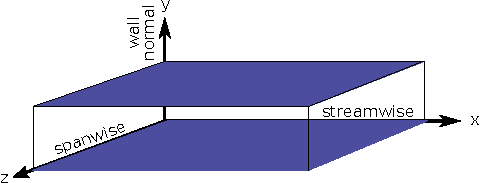
\includegraphics[height=.39\linewidth]{geometry}
%%% \caption{The Channel Geometry.}
%%%\end{center}
%%%\end{figure}
The Fourier method allows a natural decoupling between different modes
in transformed space such that multiple tasks can operate on their own data
independently. Our method uses a 2D decomposition which divides an $N_x
\times N_y \times N_z$ domain into M pencils. Fourier transforms in 3D
are performed one direction at a time, and transposes 
re-partition the domain into pencils aligned in appropriate
directions,
as depicted in Figure~\ref{fig:pencil2}. This
paper focuses on single-node performance.  Thus,
for the kernel discussed below, the final pencil depicted (x,z,y) is
the portion of the domain considered for FFT analysis on MIC.

% picture of pencils
\begin{figure}[htb]
 \begin{center}
  \includegraphics[width=0.35\textwidth]{PencilTransposeSchematic}
  \caption{The two dimensional data decomposition. The localized FFT
    on the pencil shown on the far right is ported to the KNF MIC platform.}
    \label{fig:pencil2}
 \end{center}
\end{figure}

Algorithmically, the final inverse Fourier transform, physical space
calculations, and the first Fourier transform into wavespace are
performed completely on-node and do not require MPI subroutine calls. 
Previously the inverse Fourier transform, realspace calculations,
and forward transform were performed separately. This section of code
was re-factored to perform all three steps on each line of the pencil
individually. These changes improved cache coherency and optimized the
algorithm for multithreading, the performance and scaling of which is
the basis for this section. 

The resulting FFT kernel was run with a pencil size of $\{N_x,N_z, N_y\} =$ 
(8192,1280,1), with $N_x$ corresponding to the direction being
Fourier transformed. This was iterated over six pencils to emulate
the real DNS code, which requires operating on three velocity components
($u$,$v$,$w$) as well as the non-linear terms ($uu$,$uv$,$ww$) required
to resolve the velocity at the subsequent timestep. The size of the
pencil was chosen to correspond to a realistic pencil size for a a
single compute node during a large scale DNS simulation, where the
global mesh size would be (8192,12288,1024). 

The kernel application code is written entirely in Fortran-90, and
uses OpenMP for multithreading to perform multiple 2D
FFTs simultaneously.
%and requires a series of
%two-dimensional FFTs to complete the analysis.  

We compare results from FFTW 3.3 to the FFTW interface in MKL.  Runs
were made at various thread counts on both the host Westmere and KNF
MIC platforms and the results were verified analytically. Timings were
averaged over two successive runs, and results comparing FFTW to MKL
performance are shown in
Figure~\ref{fig:mkl-vs-fftw}. Figure~\ref{fig:mkl-vs-fftw}(a) compares
the speedup factor obtained using MKL on Westmere with observed
performance increases ranging from $\sim$20-40\%.
Figure~\ref{fig:mkl-vs-fftw}(b) shows results on MIC, where the
performance increases with MKL are more dramatic, suggesting that the
FFT implementation within MKL enables more vectorization than the FFTW
counterpart. This performance difference also impacts scalability on
MIC, as shown in Figure~\ref{fig:dns_scaling}.  In this case, the
speedup factor is based on a baseline case with four threads.  The MKL
implementation scales much better than the FFTW version. With 120
threads, an overall scaling efficiency of 72\% was achieved using MKL,
whereas only 35\% was achieved with FFTW.

% completed on both the
%FFTW for Fourier transforms. The code is
%essentially a series of DO loops that iterate over the z and y
%directions. 

To quantify the impact of various runtime affinity settings available
on MIC, Figure~\ref{fig:dns_affinity} presents the real-to-complex
(Fourier transform into frequency space) performance gains for several
thread affinity options: scatter, compact or
explicit. Results in Figure~\ref{fig:dns_affinity} are
all compared against the default case: no KMP\_AFFINITY setting.
For both MKL and FFTW
linkage, the {\em scatter} setting provided the best overall
performance across a wide thread-count range.  Note that this
setting was seen to have a significant impact on observed runtimes.

%% From the provided Intel
%% documentation:
%% \begin{itemize}

%%  \item \textbf{Scatter}: ``Specifying scatter distributes the threads as
%%        evenly as possible across the entire system. scatter is the
%%        opposite of compact; so the leaves of the node are most
%%        significant when sorting through the machine topology map.'' 

%%  \item \textbf{Compact}: ``Specifying compact assigns the OpenMP thread
%%        $\langle n \rangle + 1$ to a free thread context as close as
%%        possible to the thread context where the $\langle n \rangle$
%%        OpenMP thread was placed.''

%%  \item \textbf{Explicit}:``Specifying explicit assigns OpenMP threads to
%%        a list of OS proc IDs that have been explicitly specified by
%%        using the proclist$=$ modifier, which is required for this affinity
%%        type. ''
%% \end{itemize}



% need to add discussion of affinity results here
% http://software.intel.com/sites/products/documentation/studio/composer/en-us/2011/compiler_c/optaps/common/optaps_openmp_thread_affinity.htm#Explicitly_Specifying_OS_Proc_IDS__GOMP_CPU_AFFINITY 

\begin{figure}[htp]
\begin{center}
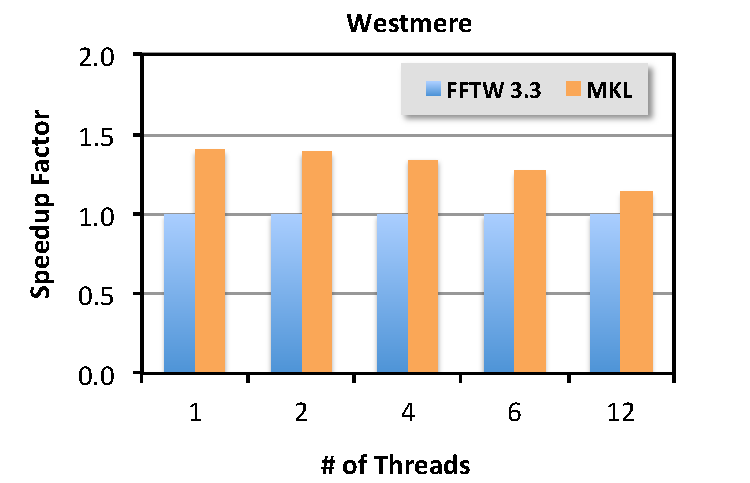
\includegraphics[width=0.95\linewidth]{dns_westmere_fftw_vs_mkl.pdf}
(a)
\includegraphics[width=0.95\linewidth]{dns_mic_fftw_vs_mkl.pdf} 
(b)
\end{center}
\vspace*{-.5cm}
\caption{Relative comparison between threaded FFT kernel
  used in DNS applications on (a) dual-socket Westmere server and (b)
  KNF MIC co-processor.}
\label{fig:mkl-vs-fftw}
\end{figure}

\begin{figure}[h]
\begin{center}
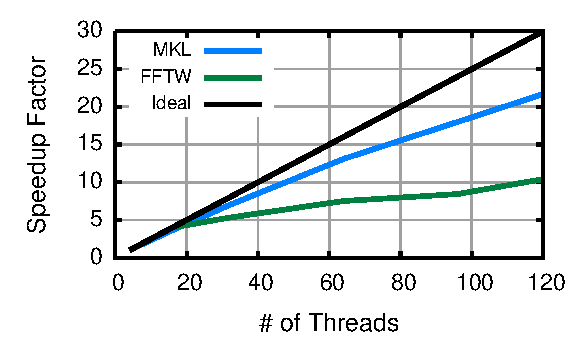
\includegraphics[width=0.9\linewidth]{dns-fftw-scaling.pdf}
\end{center}
\vspace*{-.5cm}
\caption{Scaling of DNS FFT kernel on KNF MIC accelerator ({KMP\_AFFINITY=scatter}).}
\label{fig:dns_scaling}
\end{figure}

\begin{figure}[htp]
\begin{center}
\includegraphics[width=1.0\linewidth]{dns_affinity_mkl.pdf}
(a)
\includegraphics[width=1.0\linewidth]{dns_affinity_fftw3.pdf}
(b)
\end{center}
\vspace*{-.5cm}
\caption{Influence of runtime affinity setting on MIC.
  Relative performance change is based
  on comparison to runs with no affinity setting provided. A
  positive performance change indicates faster runtimes.  Results are
  presented for FFTs performed with the (a) MKL and (b) FFTW3
  libraries.}
\label{fig:dns_affinity}
\end{figure}




%

%\begin{figure}[htp]
%\begin{center}
%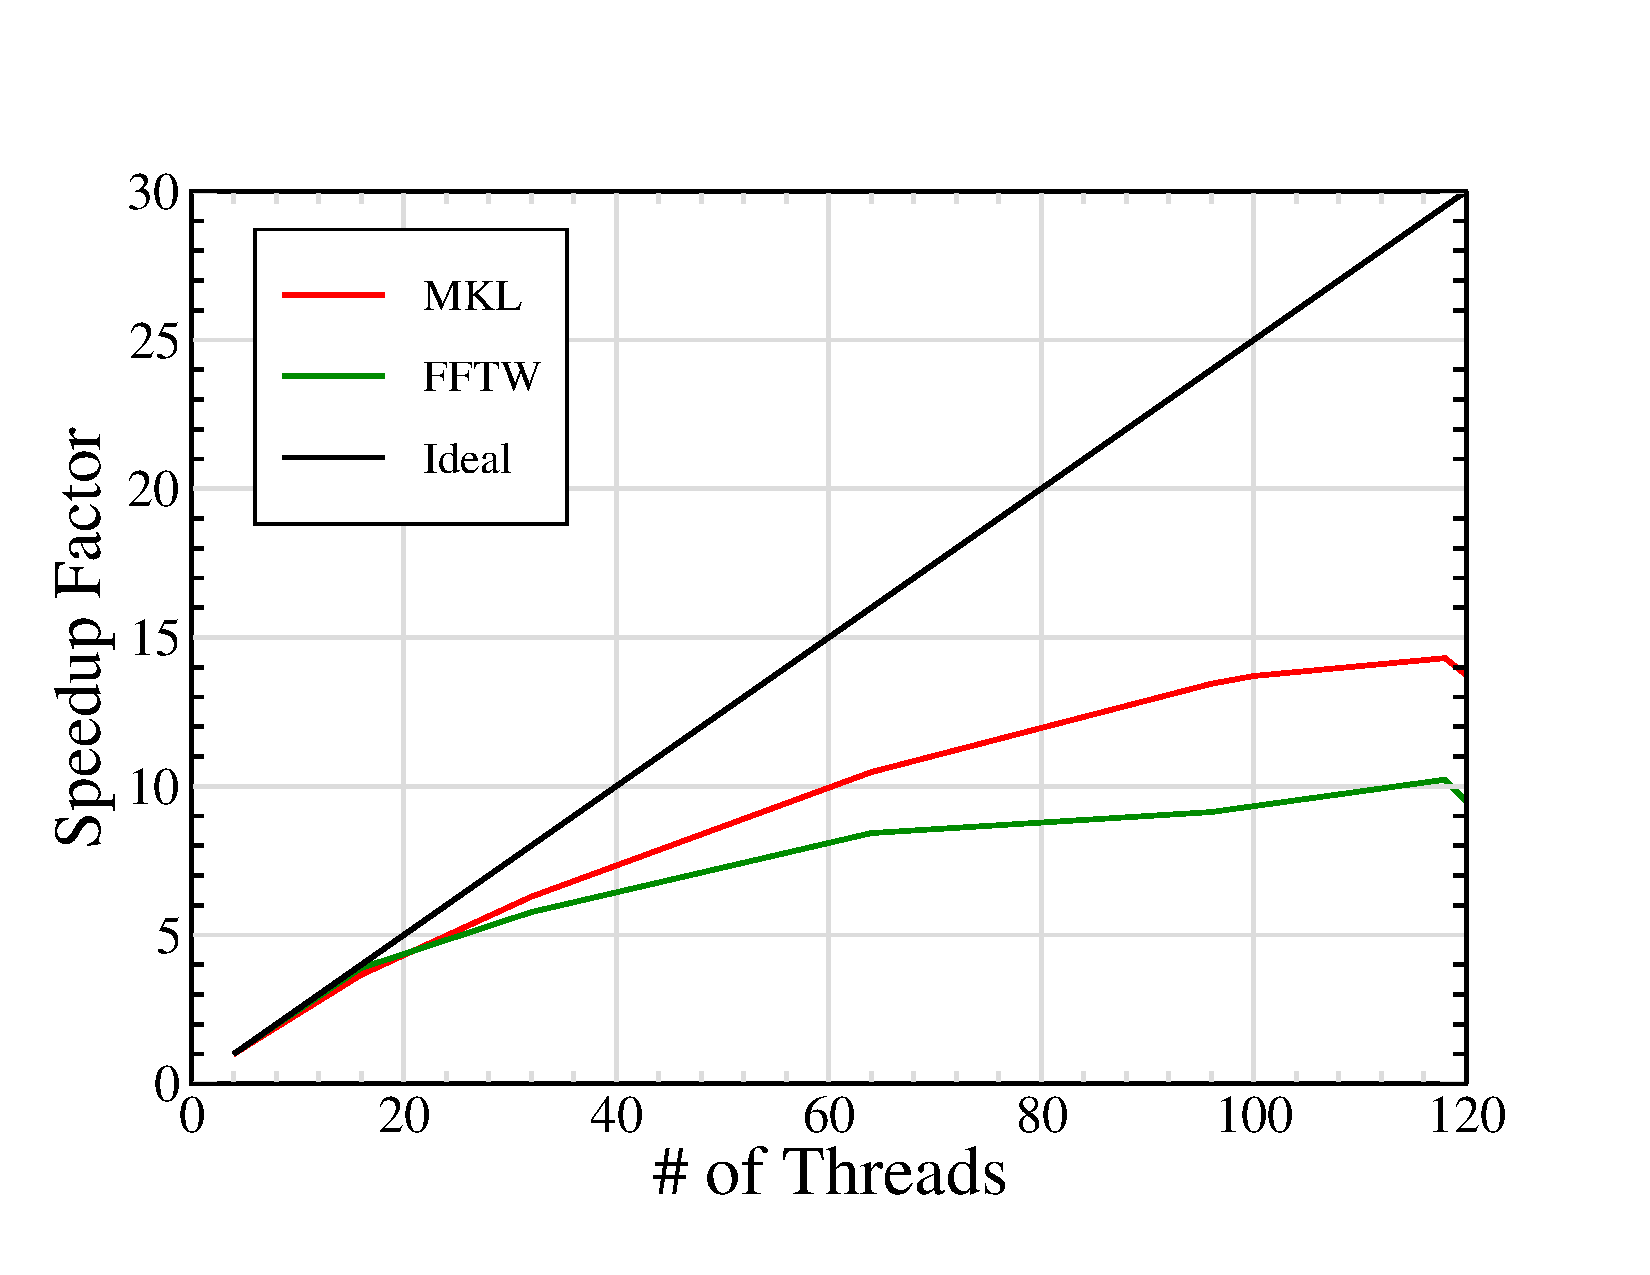
\includegraphics[width=1.0\linewidth]{dns_full_kernel.pdf}
%\end{center}
%\vspace*{-.5cm}
%\caption{Scaling of the Complex-to-Real FFT, Nonlinear computations and
% Complex-to-Real FFT DNS kernel on KNF MIC accelerator.}
%\label{fig:dns_scaling}
%\end{figure}
%
 % merging with mks section
% DNS defined in the intro!
\subsection{Incompressible DNS Application}
\label{sec:dns_full}

% Why DNS code needs to be improved
Direct numerical simulation (DNS) plays an important role in
understanding turbulent flows because DNS provides high fidelity data 
that is difficult to obtain experimentally. After Kim {\it et al.}
first used the DNS for wall-bounded turbulence flow in 1987
\cite{Kim:1987ub}, DNS has been used extensively to understand the
turbulence phenomenon and to help develop models of turbulence. 
Turbulence is characterized by a non-dimensional parameter known 
as the Reynolds Number ($Re$).  The vast majority of fluid flows 
in industry and nature occur at large $Re$. 
However, as $Re$ increases, time and length scales become smaller. 
Thus, DNS at high $Re$ naturally requires a fine meshes and time-steps 
to obtain meaningful data from flows of interest. 
Therefore, the use of state-of-art HPC systems is mandated
 to study turbulent flows of interest. To date, the highest
$Re$ of the wall-bounded turbulence DNS was at $\approx 250,000$, 
which required 242 billion degrees of freedom to 
resolve\cite{Lee:2015er}. However, $Re$ = 250,000 remains substantially 
lower than the $Re$  for many practical engineering applications. 
To enable DNS at these higher $Re$, at least exascale 
capable HPC systems are required. These systems will require
not only substantial hardware advanced, but also modifications 
to the underlying DNS codes. 

% Detail of simulation
In this section, we will show you the results of testing PoongBack on
KNL nodes in Stampede, which is a channel flow DNS code optimized for
the modern HPC systems. PoongBack,
named after the ancient Korean god of winds, 
simulates a channel flow: the flow between two infinite 
parallel plates. The simulation code
has already been scaled to several top-10 HPC systems, and has 
shown excellent performance during its use by several research 
groups\cite{Lee:2013kv}. In particular, it was used for
generating the data for the NSF supported virtual flow laboratory in the 
Johns Hopkins Turbulence Data Base\cite{Graham:2015ha}.
The code uses the Fourier-Galerkin spectral method in the streamwise and spanwise directions 
and a high-order basis spline method in the wall-normal direction. 
For time integration PoongBack uses a low-storage
third-order Runge-Kutta method\cite{Spalart:1991wu}. 
The simulation domain is partitioned by
a two-dimensional decomposition, a.k.a. pencil-decomposition. PoongBack
contains three major kernels; (1) solving the Navier-Stokes equations in
a complex domain (2) one-dimensional fast Fourier transforms (3)
data transpose in two dimension. The combination of (2) and (3) provides 3D
FFTs and there are many existing libraries for it. We developed a customized 3D
FFT library because of the needs for zero-padding for 3/2
dealiasing. Additionally, PoongBack uses a customized I/O library for the HDF-5
format, ESIO~\cite{Lee:2014ta}, which has been shown to be performant to 
large core counts, but the I/O performance is beyond the scope of the current work. 
See \cite{Lee:2013kv,Lee:2014ta} for more details about PoongBack.  

For this study the grid size used was $1024\times128\times512$, which is 
comparable to the $Re_\tau = 180$ simulation from 
Kim\cite{Kim:1987ub}. For every benchmark cases, MCDRAM is
used as a cache memory between processors and DRAM. The simulation code
was compiled with the flag ``{\tt -xMIC-AVX512}.'' \todo{should this be -ax not -x?} Also, the FFTW-3.3.5
library is installed with the options ``{\tt --enable-avx512}'' and
``{\tt --enable-mpi}.''~\cite{Frigo:2005tu}. We used double-precision
operations for all the kernels and elapsed times were measured by ``{\tt
mpi\_wtime()}'' with ``{\tt mpi\_barrier()}.'' 

\begin{figure}
 \begin{center}
   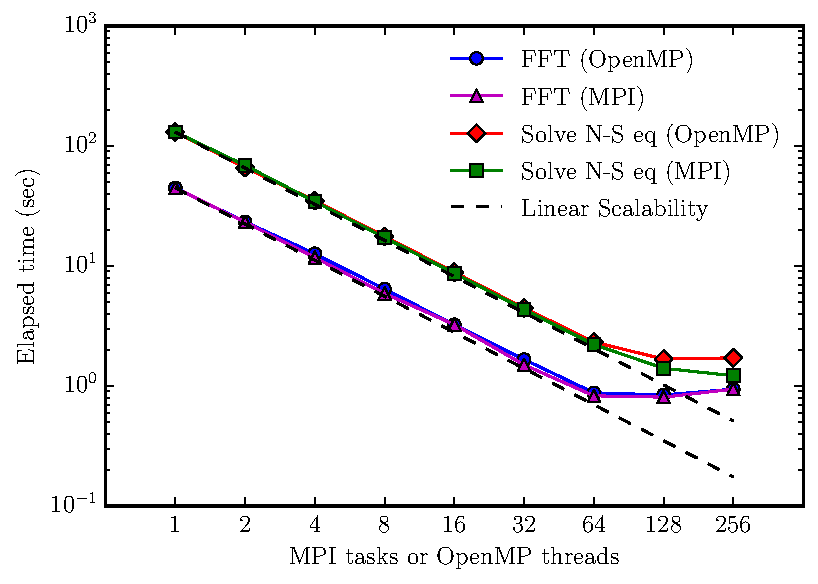
\includegraphics[width=0.45\textwidth]{DNS_FFT_Wave}
   \caption{Strong scaling result depicting 1D FFTs and the solution of the 
  N-S equations in wavespace for a single timestep.}
   \label{fig:DNS_strong_scale_fft_wave}
 \end{center}
\end{figure}

% 1D FFT and wavespace performance
Figure~\ref{fig:DNS_strong_scale_fft_wave} shows the strong scaling performance
of the kernels involving floating point operations; 1D FFTs and solving the
Navier-Stokes equations. Four different FFTs are performed; real-to-complex
(R2C), complex-to-real (C2R), forward complex-to-complex (fC2C) and backward
complex-to-complex (bC2C). Before or after each FFT, 1d contiguous data lines
are padded or truncated with zeros.  Also, nonlinear products such as $A\times
B \rightarrow C$ were performed between C2R and R2C transforms. The elapsed
time for 1D FFTs, zero padding/truncation and nonlinear product are shown in
Figure~\ref{fig:DNS_strong_scale_fft_wave} in blue and magenta. In both cases
using either MPI-only and OpenMP-only the performance is almost linear up to 64
processors. When two hardware threads were used per core (hyperthreading), the
performance did not increase. Furthermore, the performance decreases when four
hardware threads were used in both MPI and OpenMP cases. The performance was
best with 64 processors and showed 270 GFlops, or approximately 9\% of peak
performance. This means that the performance of 1D FFTs on KNL nodes are memory
bandwidth limited.

There are numerous floating point operations involved in the compute
kernels for solving the Navier-Stokes equations. 
Particularly critical numerical operations include solving the linear system  
$A \textbf{x} = \textbf{b}$, along with 
matrix-vector multiplications. The matrix $A$ is a banded matrix with
additional non-zero elements in several first and last rows. Also, the
elements of $A$ are real while the elements of $\textbf{x}$ and
$\textbf{b}$ are complex. To take advantage of these properties, we have
implemented a customized linear algebra solver. As the Navier-Stokes
equation is solved in a complex number domain, after the 1D FFTs in two
directions, the 3D PDE is decoupled and becomes a series of 1D ODEs, one
for each wavenumber. In this way, the
Navier-Stokes equations are solved concurrently at each wavenumber without
interaction between wavenumbers. As a result, this portion of the kernel
is parallelized and requires no communication. The performance of
the kernel for solving the Navier-Stokes equations is shown in
Figure~\ref{fig:DNS_strong_scale_fft_wave} in green and red. Similar to
the FFTs, both MPI-only and OpenMP-only cases were performed and show
almost ideal scalability up to 64 cores.
There were small, but noticeable, performance increases
observed with two hardware threads. Interestingly, the performance of
OpenMP only case decreases while the performance of MPI only case
increases when four hardware threads per core were applied. This could be
due to different memory access patterns between MPI and OpenMP,
or scheduling overhead in OpenMP, which was also observed in Intel's work on
HPCG\cite{Park:2014:ESI:2683593.2683696}.

% Transpose performance
\begin{figure}
 \begin{center}
   \includegraphics[width=0.45\textwidth]{DNS_Transpose}
   \caption{Strong scaling result of data reorder and MPI communication; OpenMP is not used.}
   \label{fig:DNS_strong_scale_transpose}
 \end{center}
\end{figure}

The last kernel of PoongBack is the data transpose in a two dimensionally
partitioned domain. This kernel is to ensure data alignment for FFTs and
linear problems when solving the Navier-Stokes equations and does not include
any floating point operations. However, more than 50\% of the simulation
time occurs during this operation. The data transpose kernel includes two
subsequent parts: 1) All-to-All type MPI communication in two
sub-communicators; and 2) data reordering to maximize MPI message size
and to finalize memory alignment after MPI communication. As the
domain is partitioned in two dimensions, MPI communication needs to be
performed in both dimensions. This is accomplished using MPI sub-communicators.
The communication in each direction is logically All-to-All, but other communication
patterns can be faster than ``{\tt mpi\_alltoall}'' depending on the 2D
communication topology. We have used MPI-enabled FFTW (version 3.3 or
higher), which dynamically determines the optimal communication patterns for each
sub-communicator. Since MPI-enabled FFTW only supports a one dimensionally
partitioned domain, a.k.a plane decomposition, we separately use
FFTW for 1D FFTs and MPI communications with ``{\tt
fftw\_mpi\_execute\_r2r()}'', an idea originally attributable to Dr. Rhys
Ulerich. \todo{Maybe put Rhys in the acknowledgements?} The part of code used
for data reordering performs a tensor
transpose: {\tt B(i,j,k,l) $\leftarrow$ A(l,i,k,j)} or {\tt
B(i,j,k) $\leftarrow$ A(j,k,i)}. Unfortunately, cache-line
optimization cannot be achieved for both load and store at the same
time. In this work we preferentially loaded the order of transpose. 
The performance of MPI communication and data reordering is
shown in Figure~\ref{fig:DNS_strong_scale_transpose}. Similar to the FFT
scaling and Navier-Stokes scaling in Figure~\ref{fig:DNS_strong_scale_fft_wave},
data reordering also shows nearly
perfect linear scalability up to 64 cores. Indeed, the performance
continues to increase even with hardware threading.
On the other hand, profiling the MPI communication shows performance
increases as the number of cores increases even with more than one
MPI tasks for each hardware thread. Admittedly, the scalability is far from
linear. This result is interesting because PoongBack benchmark results
on other HPC systems show that MPI communication takes more than five
times the elapsed time for data reordering~\cite{Lee:2013kv}. This
may imply that the performance could be increased by fine tuning 
the data reordering for KNL nodes. 

\begin{figure}
 \begin{center}
   \includegraphics[width=0.45\textwidth]{DNS_Parallelism}
   \caption{Comparison of MPI$\times$OpenMP in data transpose}
   \label{fig:DNS_MPI_OpenMP}
 \end{center}
\end{figure}


For data re-ordering, OpenMP can be used in each MPI task. This hybrid MPI+OpenMP parallelism
is tested and results are shown in Figure~\ref{fig:DNS_MPI_OpenMP}.
Each line in Figure~\ref{fig:DNS_MPI_OpenMP} details cases where the product of
the number of MPI tasks and the number of OpenMP threads is
constant. Using more MPI tasks and less OpenMP threads generally shows
better performance. The best performance is achieved when 256 MPI tasks
were used with four hardware threads. This is because using MPI shows
better performance than OpenMP for data reordering. Also, using more MPI
tasks performs better for MPI communication as shown in
Figure~\ref{fig:DNS_strong_scale_transpose}. 
%Finally, the size of tensor
%transpose changes with number of MPI tasks.  


\begin{figure}
 \begin{center}
   \includegraphics[width=0.45\textwidth]{DNS_full_timestep}
   \caption{Strong scaling results for the total elapsed time for single timestep. The parantheses denote: (MPI tasks $\times$ OpenMP threads). Hybrid parallelism was found to show the best performance, with nearly perfect scalability until approximately 128 concurrencies.}
   \label{fig:DNS_strong_scale_total_elapsed_time}
 \end{center}
\end{figure}

The performance of one full timestep (without I/O) is shown in
Figure~\ref{fig:DNS_strong_scale_total_elapsed_time}. The best
performing set of MPI $\times$ OpenMP concurrency for each number of 
processors was chosen. It also shows almost perfect scalability up to 64
processors. The performance continues to increase after using hardware
threads. In most cases, using only MPI tasks shows the best performance, 
excepts at 64 processors with 2 hardware threads. However, the
difference between hybrid parallelism and only MPI tasks are minimal at
128 processors. A conclusion from this study is that generally speaking, 
using only MPI seems to be the best option for any problem size. 
Despite this, we also note that hybrid parallelism could be more 
important due to the off-node impact. When the problem size
is bigger than the size of DRAM on a KNL node, one must use multiple KNL
nodes. Using many MPI tasks can easily saturate the capability of
the interconnect device. Under these conditions, reducing the number of MPI tasks
by using OpenMP would likely improve performance.   

%\todo{if we merge this with the previous section, we can have an intro
%to dns and then talk about each in detail}
% NM-- done

% DNS defined in the intro!
\subsection{Gaussian processes}
\label{sec:chol}

It is common in many uncertainty quantification applications to replace an
expensive model, possible a discretised partial differential equation with a
cheap surrogate.  This is done so that during a Markov chain Monte Carlo
procedure, likelihood evaluations are cheap.  There are a plethora of different
surrogate choices and strategies for choosing which is appropriate for a
particular application.  Gaussian processes are a common choice, and we explore
their scaling on the KNL architecture here.

\todo{hierarchical!!!}

Gaussian processes are a probabilistic model for generating random fields
characterised by a mean function and a covariance function.
\begin{equation}
  f(x) \sim \mathcal{N}(\mu(x), c(x, x'))
\end{equation}

They have the property that evaluation of the field at some finite set of
points $(x_1, \ldots, x_n)$ yields a multivariate normal vector with a known
mean vector and symmetric and positive-definite covariance matrix
\begin{equation}
  \begin{pmatrix}
    f(x_1) \\
    \hdots \\
    f(x_n)
  \end{pmatrix}
  \sim \mathcal{N}(\mu, \Sigma).
\end{equation}
Thus, laying down a grid of points we wish to model the field at yields the
usual Gaussian probability distribution function we are familiar with,
\begin{equation}
  p(x) \propto |\Sigma|^{-1/2} \exp(-\frac12 x^\top \Sigma^{-1} x).
\end{equation}
Notice that evaluation of this probability density function necessitates a
linear solve $\Sigma u = x$.  Since $\Sigma$ is symmetric and positive-definite
a Cholesky factorisation is required.  Iterative approaches exist too, but we
concentrate on the direct approach here.  It is also worth noting that the
covariance function is typically takes an exponential form
\begin{equation}
  c(x, x') = \sigma^2 \exp(-\frac12 \| x - x' \|^2 / l^2)
\end{equation}
and so the resulting covariance matrix
\begin{equation}
  \Sigma_{ij} = c(x_i, x_j)
\end{equation}
is very commonly full and dense.  The usual approach is taken for evaluation
of the probability density function
\begin{enumerate}
  \item Compute $L$ such that $\Sigma = LL^\top$.
  \item Solve $\Sigma u = x$ using 1.
  \item Compute the inner-product $x^\top u$.
  \item Divide by the square root of the determinant of $\Sigma$.
  \item Return $p$
  \item Go to 1. for the next state in the Markov chain.
\end{enumerate}

QUESO was used to manage the Gaussian process and Markov chain infrastructure.
The meat of the heavy lifting is done inside the likelihood evaluation which
necessitates the evaluation of the Gaussian probability density function.
Extensive use of Intel's MKL was used for both the Cholesky factorisation and
subsequent linear solve.

\missingfigure{Strong scaling of the GPs on a single MIC (e.g. problem size
constant and increasing number of threads)}

Some discussion is warrented: is this ameniable to MICs? Vs typical CPUs?

% DNS defined in the intro!
\subsection{Blended Isogeometric Discontinuous Galerkin (BIDG) Method}
\label{sec:isogeometric}

For the scaling study the blended isogeometric discontinuous Galerkin (BIDG) code, ArcSyn3sis is used.  The BIDG algorithm was developed in \cite{Michoski2016658} to exploit and seamlessly merge key capabilities offered by both isogeometric analysis and discontinuous Galerkin methods. This method is an inherently high-order method that is amenable to $hp$-adaptive schemes, and shows requisite super-exponential convergent behavior.

In traditional isogeometric analysis tight coupling between computer aided design (CAD) mesh automation tools for complex geometric domains, such as jet engines and tokamak fusion reactors, has been developed for triangles in two dimensions \cite{Engvall2016378}, and generalized elements in three dimensions \cite{EngvallPress}.  This allows for meshes that exactly preserve underlying geometry in real-world mesh designs, including arbitrarily smooth and discontinuous features.  In many application, geometric sensitivities are known to dominate errors, and as such having high-order accurate solutions on geometrically consistent meshes is essential.


\begin{figure}[h]
\begin{center}
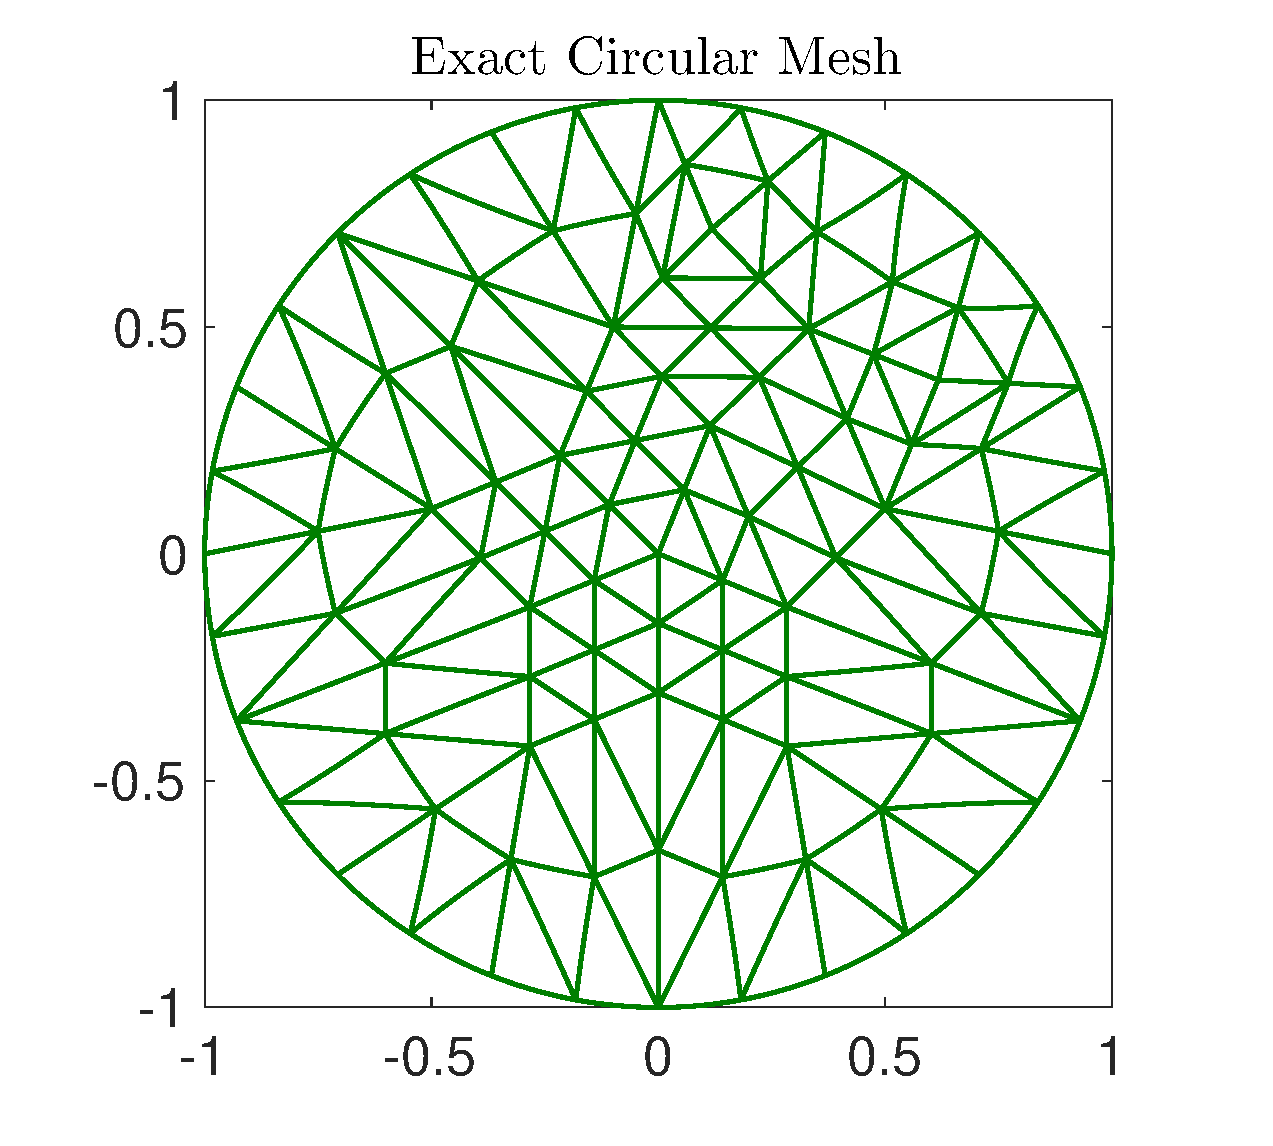
\includegraphics[width=0.8\linewidth]{./bidg_data/168_circ}
\end{center}
\vspace*{-.5cm}
\caption{Exact b\'{e}zier circular mesh used in the scaling study.}
\label{fig:dns_scaling}
\end{figure}


The discontinuous Galerkin method, on the other hand, excels in aspects of its computational efficiency in the context of modern architectures, particular in convection-dominated flows that allow for localization of finite element stencils in such a way that dynamic problems lead to block diagonal matrix systems.  The locality of the memory footprint in these application models leads to the ability to compute at high local order at unusally high arithmetic intensity \cite{Klöckner2009786}.

The BIDG method merges these two methods seamlessly by utilizing a peicewise rational isogeometric basis for the geometry, and a peicewise discontinuous polynomial representation for the model, while providing an exact (and properly conditioned) geometric transformation between the two spaces  \cite{Michoski2016658}.

For our scaling test here we solve the first-order acoustic wave equation: \begin{equation} \label{awe} \frac{\partial p}{\partial t} + \nabla\cdot \boldsymbol{u} = 0, \quad  \frac{\partial\boldsymbol{u}}{\partial t} + \nabla p = 0, \end{equation} where $\boldsymbol{u}=(u_x,u_y)$ is the velocity, and $p$ the pressure.

Broadly such a system is discretized by solving the semidiscrete block diagonal system \[ \left( v, \frac{ \partial A}{\partial t} \right)_{\Omega_{i}}= V_{\Omega_{i}}+S_{\partial\Omega_{i}} \] for $A = (p,\boldsymbol{u})$, $V_{\Omega_{i}}$ a volume kernel that has only elementwise dependencies, and $S_{\partial\Omega_{i}}$ a surface kernel that depends on interelement communication through classical upwinding \cite{Michoski2014898}.  


\begin{figure}[h]
\begin{center}
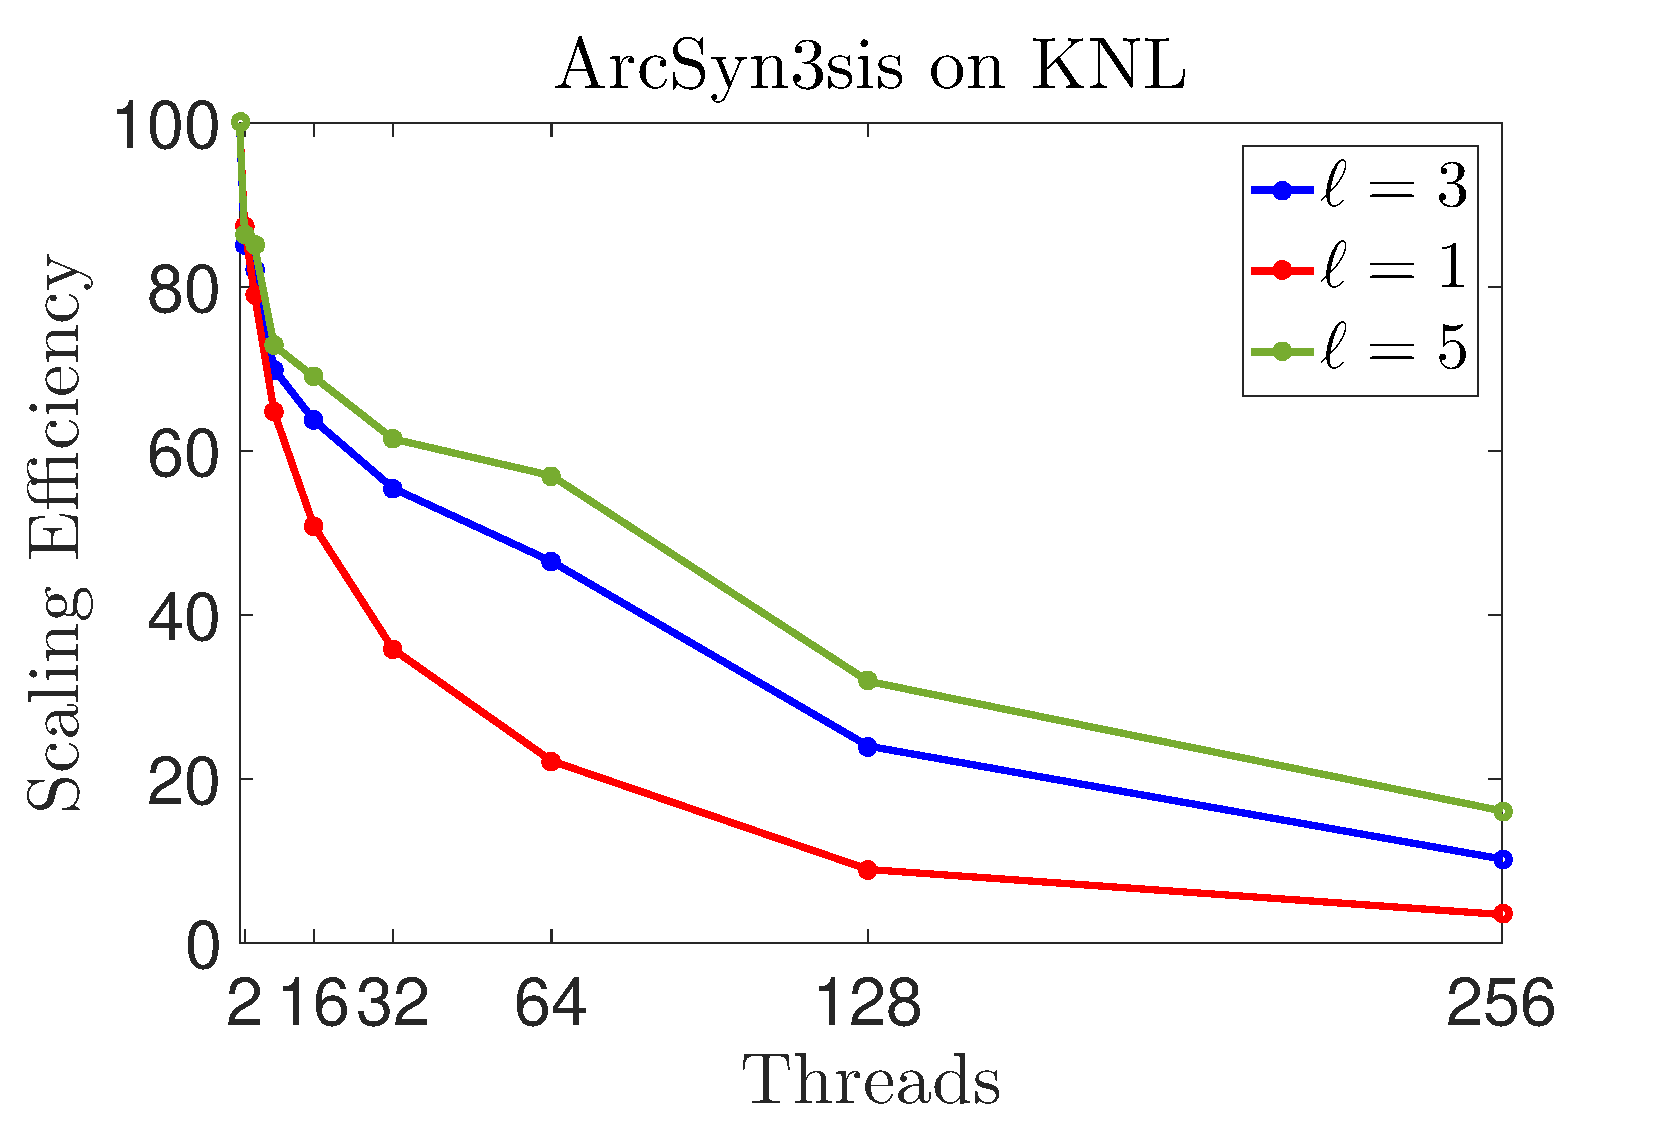
\includegraphics[width=0.95\linewidth]{./bidg_data/scaling_p}
\end{center}
\vspace*{-.5cm}
\caption{Strong scaling of the ArcSyn3sis BIDG kernel on KNL nodes run on isogeometric 168 element mesh, and shown at different element order $\ell$.}
\label{fig:bidg_scaling}
\end{figure}


The implementartion on isogeometric meshes utilizes the Open Concurrent Compute Abstraction (OCCA) library \cite{MedinaPress}.  The library uses an off-load model for abstracting back-ends and kernel libraries from OpenMP, OpenCL, and CUDA using a C-based macros approach.  The OCCA kernel implements macro-based just-in-time code generation so that the platform target can be identified at runtime.  Threaded barriers are also set in the application kernel to allow for thread-based granularity, giving more flexibility during code optimization.  The implementation of the ArcSyn3sis kernel allows for aliasing of flattened arrays, such that the data structures can be called more intuitively (e.g. a 4-tensor can be called as a four array, instead of indexed as a flattened contiguous one array).  The volume kernel can be written in three nested loops; the outer looping over elements, and two inner loops over degrees of freedom in the DG basis.  The surface kernel similarly loops over elements, but then due to an additional interpolation step form the isogeometric transformation, extends one of these nested loops over the quadrature degrees of freedom for curved edges.

The results of the basic scaling study are shown in Fig.~\ref{fig:bidg_scaling}.  These priliminary results seem to indicate improved scaling as a function of polynomial order $\ell$, which is consistent with the theoretical behavior of the algorithmic intensity of DG algorithms.  However, this is clearly not enough evidence to be certain that such scaling is being observed.  In particular, on this mesh we see an efficiency saturation above $\ell>5$.  Moreover, since the mesh itself has only 168 elements, the number of threads eventually exceeds the number of elements, making for some intriguing questions regarding the observed behavior.  In order to fully understand the current, a more extensive study is required, including a streams benchmark \cite{McCalpin1995} and roofline performance test \cite{Williams:2009:RIV:1498765.1498785}.


%
% NM --- feel free to disregard anything I recommend here
%
 %yar\todo{Discuss, broadly, what class of problems this resides in and why humanity works on it}

%% yar2\todo{some basic intro to the linear algebra you are doing}

%% yar3\todo{any nuances of porting to MIC?}

%% yar4\todo{discussion of scalability observed}

%% \missingfigure{Strong scaling of the GPs on a single MIC (e.g. problem size constant
%% and increasing number of threads)}

%Finally, some discussion is needed: is DG ameniable to MICs? Vs typical CPUs? I
%naively guess so, since you can essentially vectorize several of the
%activities.


\subsection{EOM-CCSDT single-node performance}
\label{sec:cfour}

For the calculations used in this work,
the CFOUR \cite{cfour:08} program was used. CFOUR
(Coupled-Cluster techniques for Computational Chemistry) is an
application for performing high-level quantum chemical calculations
that is under active development by research groups at UT Austin and
Universit\"{a}t Mainz, Germany). CFOUR's major strength is its arsenal
of high-level ab initio methods for the calculation of atomic and
molecular properties.  Virtually all approaches based on M\o
ller-Plesset (MP) perturbation theory and the coupled-cluster
approximation (CC) are available.

For the other applications considered here, the scalibility of various code bases 
used in the PECOS center on KNL compute nodes has been presented. To compliment
this effort, this section will focus on a comparison of optimal single-node performance
between traditional (Haswell) Intel CPUs and the new KNL compute nodes of Stampede 2.
While the scalability of CFOUR on current and emerging architectures will be the focus 
of future work, the results presented here will detail overall runtime performance gains
from migrating to this new architecture. 

For this work, the performance of a single calculation, the EOM-CCSDT energy of the first
excited singlet state of $C_2H_2$, was studied in detail. This excited state is the focus
of a current study being conducted by authors of this paper in which over 1 million single point
energies will be calculated. As such, ensuring the best performance for this run type will conserve
important national compute resources available at TACC. All EOM-CCSDT calculations were performed 
using the NCC module \cite{ncc:15} of the CFOUR program system 
and the ANO1 basis set \cite{ano1:87} with core electrons uncorrelated. A nonequilibrium geometry
of this excited singlet state was used that has C1 symmetry. The lowest symmetry point group available to 
$C_2H_2$ was used because this computational requires the most memory and compute time. This establishes
an upper bound per computation.

Porting CFOUR to the KNL architecture was very straightforward. No modification of the code or the build
system was required. All that needed to be done was to add the previously discussed compile and link flags
to the corresponding Fortran, C, and C++ environmental variables.

The NCC module in CFOUR is a recent contribution to the code and, as such, has been designed to take
advantage of many-core architectures. It uses OpenMP for thread-based parallelism and in this work, the
built-in parallelism of Intel's MKL is also exploited. As has been discussed in detail previously \cite{ncc:15},
it has been determined that on traditional dual Intel CPU compute node systems, best performance is obtained 
by using $OMP\_NUM\_THREADS=16$. This relies on the default behavior that MKL will use $OMP\_NUM\_THREADS$ 
if outside an OpenMP block but run single-threaded within an OpenMP block. In the NCC module, there are MKL-library 
calls within an OpenMP block, however, best performance is achieved by using only serial MKL calls within OpenMP
blocks. This ensures that thread oversubscription never occurs.

For benchmark comparison purposes, the traditional CPU used for reference was an Intel Xeon  E5-2670 v3 CPU
running at 2.30GHz. This CPU was first available on market in late 2014 and is representative of typical HPC 
compute nodes in current generation supercomputers. Best performance on this system was achieved with 
$OMP\_NUM\_THREADS=16$ and the total compute time for the $C_2H_2$ excited state energy discussed previously
was 607 s. If more than 16 threads were used, the total walltime for the calculation increases.

\subsubsection{memory mode and membind}
\subsubsection{cluster mode}
\subsubsection{threads and mkl and environmental variables oh my}
\subsubsection{cfour conclusion}

\section{Summary}
\label{sec:summary}

Using hardware that will appear in the upcoming Stampede 2 cluster, we studied
the ease of portability of a diverse set of scientific software packages to
KNL.  The software packages used in this paper were written in a variety of the
most commonly used procedural languages and are workhorses for solving problems
in many disciplines of computational science.

Overall, our experiences porting scientific applications to the KNL
architecture were positive.  Software at PECOS typically ships with a
flexible build system and customizing compiler flags for a KNL-specific
instruction set is simple.  Furthermore, we observed that KNL compute nodes can
deliver impressive compute power and scalability for relatively little human
effort.  Contrasting this with experiences on previous generations of Intel
Xeon Phi MICs~\cite{schulz2012early}, it is clear bootable MICs that do not
require code intervention for offloading onto co-processor MICs such as Knights
Ferry yield a much larger performance-to-effort ratio for computational
scientists.

We note that although KNL has several boot-time options that specify memory
hierarchy and layout, Intel's recommended default cluster mode, Quadrant, along
with the Cache memory mode brings most of the benefits of performant memory access 
and bandwidth without the drawbacks of explicitly management through ``numactl''.

Lastly, in addition to strong scaling results on KNL, we have presented some
promising runtime comparisons with traditional Haswell Xeon E5-2670 CPUs.

% Performance results vary more widely.  We have demonstrated good strong scaling
% to large thread counts for some of our computational kernels, but others only
% effectively used a fraction of the MIC's potential capability.  However,
% runtime performance seldom degraded for large thread counts on all workloads,
% and simple changes to thread algorithms or affinity settings often delivered
% further improvements.  Different workloads require different settings in order
% to achieve peak performance. Finally, vectorization is critical to fully
% exploit the MIC architecture.



\begin{acks}
The authors acknowledge the Texas Advanced Computing Center (TACC) at The
University of Texas at Austin for providing HPC resources that have
contributed to the research results reported within this paper.
\end{acks}

\bibliographystyle{ACM-Reference-Format}
\bibliography{c,mk,damon,csim}

\end{document}
